
\chapter{Dosáhneme kolektivní imunity o\v{c}kováním?} \label{Nekolik_poznamek}

\textit{Martin Šmíd}
\vspace{15mm}

\section*{Úvod}

\noindent Očkování je zatím nejúčinnějším a zároveň jedním z~nejméně kontroverzních pro\-střed\-ků boje proti současné pandemii. Čím více lidí bude naočkováno,
tím více stávajících opatření může být zrušeno, a pokud bude dosaženo určité kritické meze, v~principu nebude potřeba žádných opatření. V~epidemickém modelování se zmi\-ňo\-va\-né kritické mezi říká {\em práh kolektivní imunity} a vypočítá se jako $H=\frac{1}{R_0}$, kde $R_0$ je základní reprodukční číslo. Proč se $H$ vypočítá právě takto, je nasnadě: pokud je vůči infekci místo celé populace vnímavý pouze její poměr $h$, potom každý infekční jedinec nakazí místo $R_0$ osob pouze $h R_0$, takže při $h < H$ epidemie postupně vymizí. V~našem případě je situace složitější, protože vakcína neposkytuje stoprocentní ochranu a kromě toho je třeba vzít v~úvahu, že určitá část populace je imunní díky prodělané nemoci. Navíc je reprodukční číslo v~praxi uměle snižováno protiepidemickými opatřeními, na druhou stranu se nakažlivost SARS-CoV-2 kvůli mutacím postupně zvyšuje. 

Tato kapitola si klade za cíl vzít v potazvšechny tyto faktory a odhadnout, jaký poměr populace je potřeba očkovat, aby výsledkem byl útlum epidemie.
Protože jsou vstupy naší analýzy předmětem značné nejistoty, její výsledky jsou nejistotou nutně zatíženy a jako takové je nutno je brát. Přesto se domníváme, že naše výsledky mohou do problematiky vnést určité nové světlo. Ukazují například, že potřebná míra vakcinace ani příliš nezávisí
;na promořenosti populace, ani na údajném sezónním chování epidemie,
tedy na faktorech, které bývají často uváděny jako něco, co epidemii samo utlumí, takže očkování ztratí smysl.

\section*{Model}

V~souladu s~hlavním proudem epidemiologického modelování předpokládejme, že reprodukční číslo epidemie (tj. 
počet osob, které v~průměru nakazí jeden infekční jedinec) závisí na počtu jeho
rizikových kontaktů, úrovni imunity populace, míře ochranných opatření
nesouvisejících přímo s~počtem kontaktů a základním reprodukčním
číslem, tj. středním počtem osob, které by se od jednoho infekčního jedince nakazily, kdyby nebyl
nikdo imunní a nebyla by zavedena žádná opatření nákazu omezující. Pro jednoduchost
předpokládáme, že je tato závislost multiplikativní: 
\begin{equation}
R_{t}\doteq r_{t}\times C_{t-2}\times I_{t},\qquad r_{t}=R_{t}^{0}\times P_{t},
\label{eq:r}
\end{equation}
kde $R_{t}$ je reprodukční číslo v~týdnu $t$, $C$ je redukce rizikových kontaktů,
$I$ je redukce nakažlivosti daná vakcinací nebo imunitou, získanou
po prodělání onemocnění, $R^{0}$ je základní reprodukční číslo a
$P$ je vliv opatření přímo nesouvisejících s~redukcí kontaktů (roušky, hygiena, opatrnost, ale i trasování, které efektivně snižuje dobu, po kterou je člověk infekční).\footnote{V řeči značení, běžně používaného pro SIR modely, lze vztah (\ref{eq:r}) ekvivalentně vyjádřit jako 
$$ 
R = r_\beta \times \beta \times r_c \times \frac{S}{N} \times \frac{1}\gamma = r_\beta \times r_c \times \frac{S}{N} \times R_0,
$$
kde $r_c$ je redukce kontaktů (odpovídá našemu $C$), $r_\beta$ je redukce nakažlivosti (odpovídá $P$), $S$ je počet vnímavých jedinců v~populaci, $N$ je celková velikost populace, $\beta$ a $\gamma$ jsou parametry SIR modelu a $R_0$ je základní reprodukční číslo, viz též kapitolu \ref{Typy_modelu}.} Hodnota $r_t$ se dá interpretovat jako základní reprodukční
číslo se zohledněním dodatečné ochrany $P_{t}$. Rovnici (\ref{eq:r}) dále použijeme dvojím způsobem: nejprve z~historických dat odhadneme trend $r_t$, poté za použití tohoto odhadu pomocí rovnice určíme míru vakcinace potřebnou pro utlumení epidemie.

Hodnoty reprodukčního čísla $R$ počítáme takzvaným zjednodušeným způsobem, v~našem případě jako podíl týdenního přírůstku mezi čtvrtky daného a minulého týdne a týdenního přírůstku pět dní předem, tj. mezi sobotami minulého a před\-mi\-nu\-lé\-ho týdne \cite{Rodhad}. Výhodou tohoto způsobu výpočtu je jednoduchost, intuitivnost, závislost pouze na jednom parametru (reprodukční doba) a robustnost vůči týdenním fluktuacím a vůči změně podílu
odhalených nakažených (ascertainment rate), jehož případný skok vychýlí
maximálně dvě týdenní pozorování.

Redukci kontaktů $C$ odhadujeme pomocí průměrného počtu rizikových
kontaktů uváděného longitudinálním výzkumem \cite{paqcovid}. Dvoutýdenní zpoždění bylo zvoleno na základě faktu, že právě při tomto zpoždění je dosažena nejlepší korelace mezi $R$ a $C$, viz kapitolu \ref{Co_na_cem_zavisi}, bod 4. 

Pro jednoduchost považujeme získanou imunitu za stoprocentní u~všech,
kdo nemoc prodělali (připomeňme, že velká většina hlášených případů
nastala do sedmi měsíců před vznikem tohoto textu). Dále předpokládáme,
že ti, kteří obdrželi před více než třemi týdny první dávku vakcíny,
jsou imunní s~pravděpodobností $e^{1}=0.7$, zatímco ti, kteří jsou
týden a déle po druhé dávce, jsou imunní s~pravděpodobností $e^{2}=0.85$.
Tyto hodnoty jsme převzali ze studie \cite{Hall_etal2021} efektivnosti
vakcíny Comirnaty (Pfizer/BionTech), kterou obdržela většina očkovaných
v~České republice. 

Ve své analýze reflektujeme fakt, že určitá část infekcí nebyla
hlášena, konkrétně že pravděpodobnost hlášení infekce (ascertainment
rate) je $\alpha=0.4$ (tento odhad je diskutován níže). Z~výše uvedeného vychází,
že podíl těch, kteří nejsou v~čase $t$ imunní, je roven:
\begin{equation}
I_{t}=\left(1-\frac{x_{t}}{\alpha}\right)\left(1-v_{t}\right),\qquad v_{t}=(\pi_{t}^{1}-\pi_{t}^{2})e^{1}+\pi_{t}^{2}e^{2},\label{eq:i}
\end{equation}
kde $x$ je podíl populace s~hlášenou infekcí, $\pi^{1}$ je podíl počtu osob nejméně tři týdny po první dávce vůči počtu osob bez hlášené infekce a $\pi^{2}$ je podíl osob
nejméně týden po druhé dávce vůči počtu osob bez hlášené infekce. Hodnoty $x$ a $\pi$ jsme určili pomocí údajů z~veřejné databáze Ministerstva
zdravotnictví ČR \cite{mzcrdata}.\footnote{Ke vztahu (\ref{eq:i}) jsme došli následujícím způsobem: podle nařízení \cite{covidportalspec} nelze 90 dní po prodělání nemoci očkovat a též se dá předpokládat, že lidé, kteří nemoc prodělali, se očkovat spíše nebudou. Zdá se tedy rozumné předpokládat, že ti, kteří prodělali hlášenou infekci, se neočkují, zatímco u~těch, kteří hlášenou infekci neprodělali, fakt očkování nezávisí na tom, zda infekci (skrytě) prodělali či nikoli. Potom máme 
\begin{multline*}
I~= \mathrm{P}[\text{vnímavý}]= \mathrm{P}[\text{vnímavý}|\text{hlášen}]\mathrm{P}[\text{hlášen}]
+\mathrm{P}[\text{vnímavý}|\text{nehlášen}]\mathrm{P}[\text{nehlášen}]
\\
= 0 \times \mathrm{P}[\text{hlášen}] 
+ \mathrm{P}[\text{neprodělal nemoc ani není chráněn vakcínou}|\text{nehlášen}]\mathrm{P}[\text{nehlášen}]
\\
= 0+\mathrm{P}[\text{neprodělal nemoc}|\text{nehlášen}]\mathrm{P}[\text{není chráněn vakcínou}[\text{nehlášen}]\mathrm{P}|\text{nehlášen}]
\\
= \frac{1-\frac{x_{t}}{\alpha}}{1-x_t}\left(1-v_{t}\right)(1-x_t)=\left(1-\frac{x_{t}}{\alpha}\right)\left(1-v_{t}\right)´,
\end{multline*}
protože
\begin{multline*}
\mathrm{P}[\text{chráněn vakcínou}[\text{nehlášen}]\\=\mathrm{P}[\text{má jednu dávku}[\text{nehlášen}]e^1+\mathrm{P}[\text{má obě dávky}[\text{nehlášen}] e^2.
\end{multline*}
}

Obrázek \ref{fig:rci} znázorňuje vývoj veličin $R$, $C$ a $I$.
\begin{figure}
\begin{center}
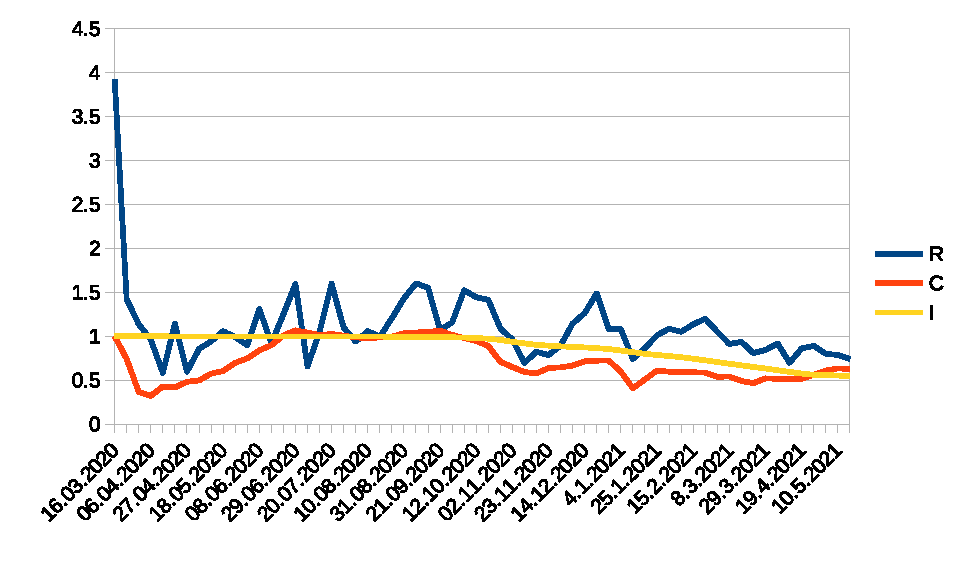
\includegraphics[scale=0.4]{pic/rc}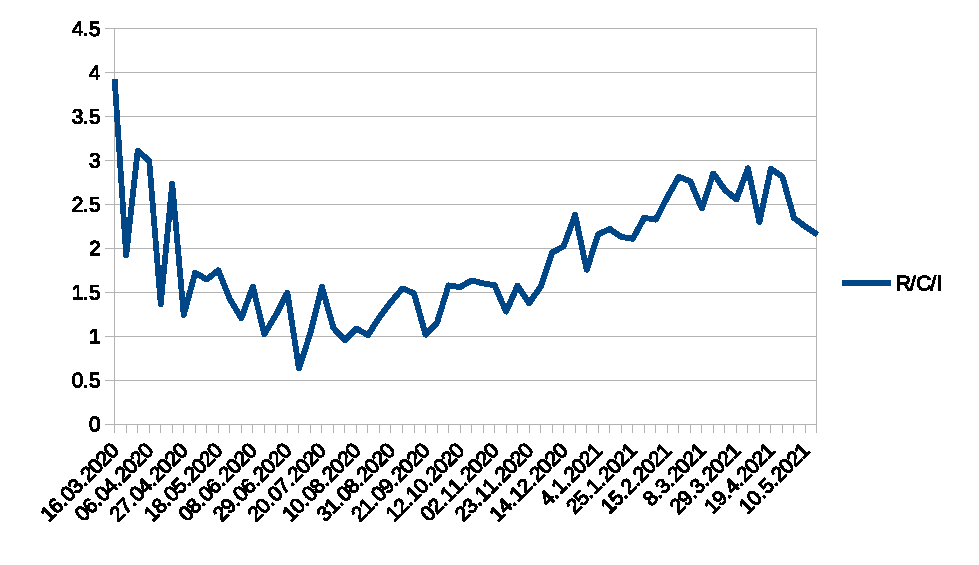
\includegraphics[scale=0.4]{pic/rci}
\caption{Vlevo: historie zjednodušeného reprodukčního čísla $R$, redukce kontaktů $C$ a míry vnímavé populace $I$. Vpravo: $\hat{r} = \frac{R_{t}}{C_{t-2}I_t}$ (odhad $r$).} 
\label{fig:rci}
\end{center}
\end{figure}
Levý graf zobrazuje časový průběh všech tří veličin, pravý pak veličinu
$\hat{r}_t = \frac{R_{t}}{C_{t-2}I_{t}}$, která je přirozeným odhadem $r_{t}$
(viz (\ref{eq:r})). Na první pohled svědčí průběh této 
křivky pro silný sezónní vliv -- v~létě jsou hodnoty značně
nižší než v~zimě. My sezónnost pro jednoduchost v~prv\-ním přiblížení nepředpokládáme -- je totiž také možné, že nižší hodnoty
$r$ jsou zdánlivé: nákaza v~letním období nebyla komunitní a v~ohniscích,
kde propukla (důl Darkov \cite{darkov} či Církvice u~Kutné Hory \cite{cirkvice}),
byla zavedena opatření omezující kontakty, která však nebyla reflektována
celostátním výzkumem \cite{paqcovid}.
Vysoké hodnoty odhadu $\hat r$ z~počátku první vlny
epidemie by se pak daly interpretovat jako následek počáteční nulové dodatečné
ochrany $P_{t}$, je však třeba si též uvědomit, že systém sběru
dat se teprve zabíhal, do testování bylo zapojeno menší množství laboratoří, navíc byly počty nakažených velice malé, data
tedy mohla být zkreslena náhodnými fluktuacemi. Protože však pro uvažování seóonnosti existují přesvědčivé argumenty, zejména fakt, že se více rizikových kontaktů odehrává v uzavřených prostorách, dále v článku uvažujeme i~model se sezonní složkou.

Graf na obrázku \ref{fig:xy} zobrazuje hodnoty $R_{t}$ vykreslené oproti násobku
$C_{t-2}\times I_{t}$. 
\begin{figure}
\begin{center}
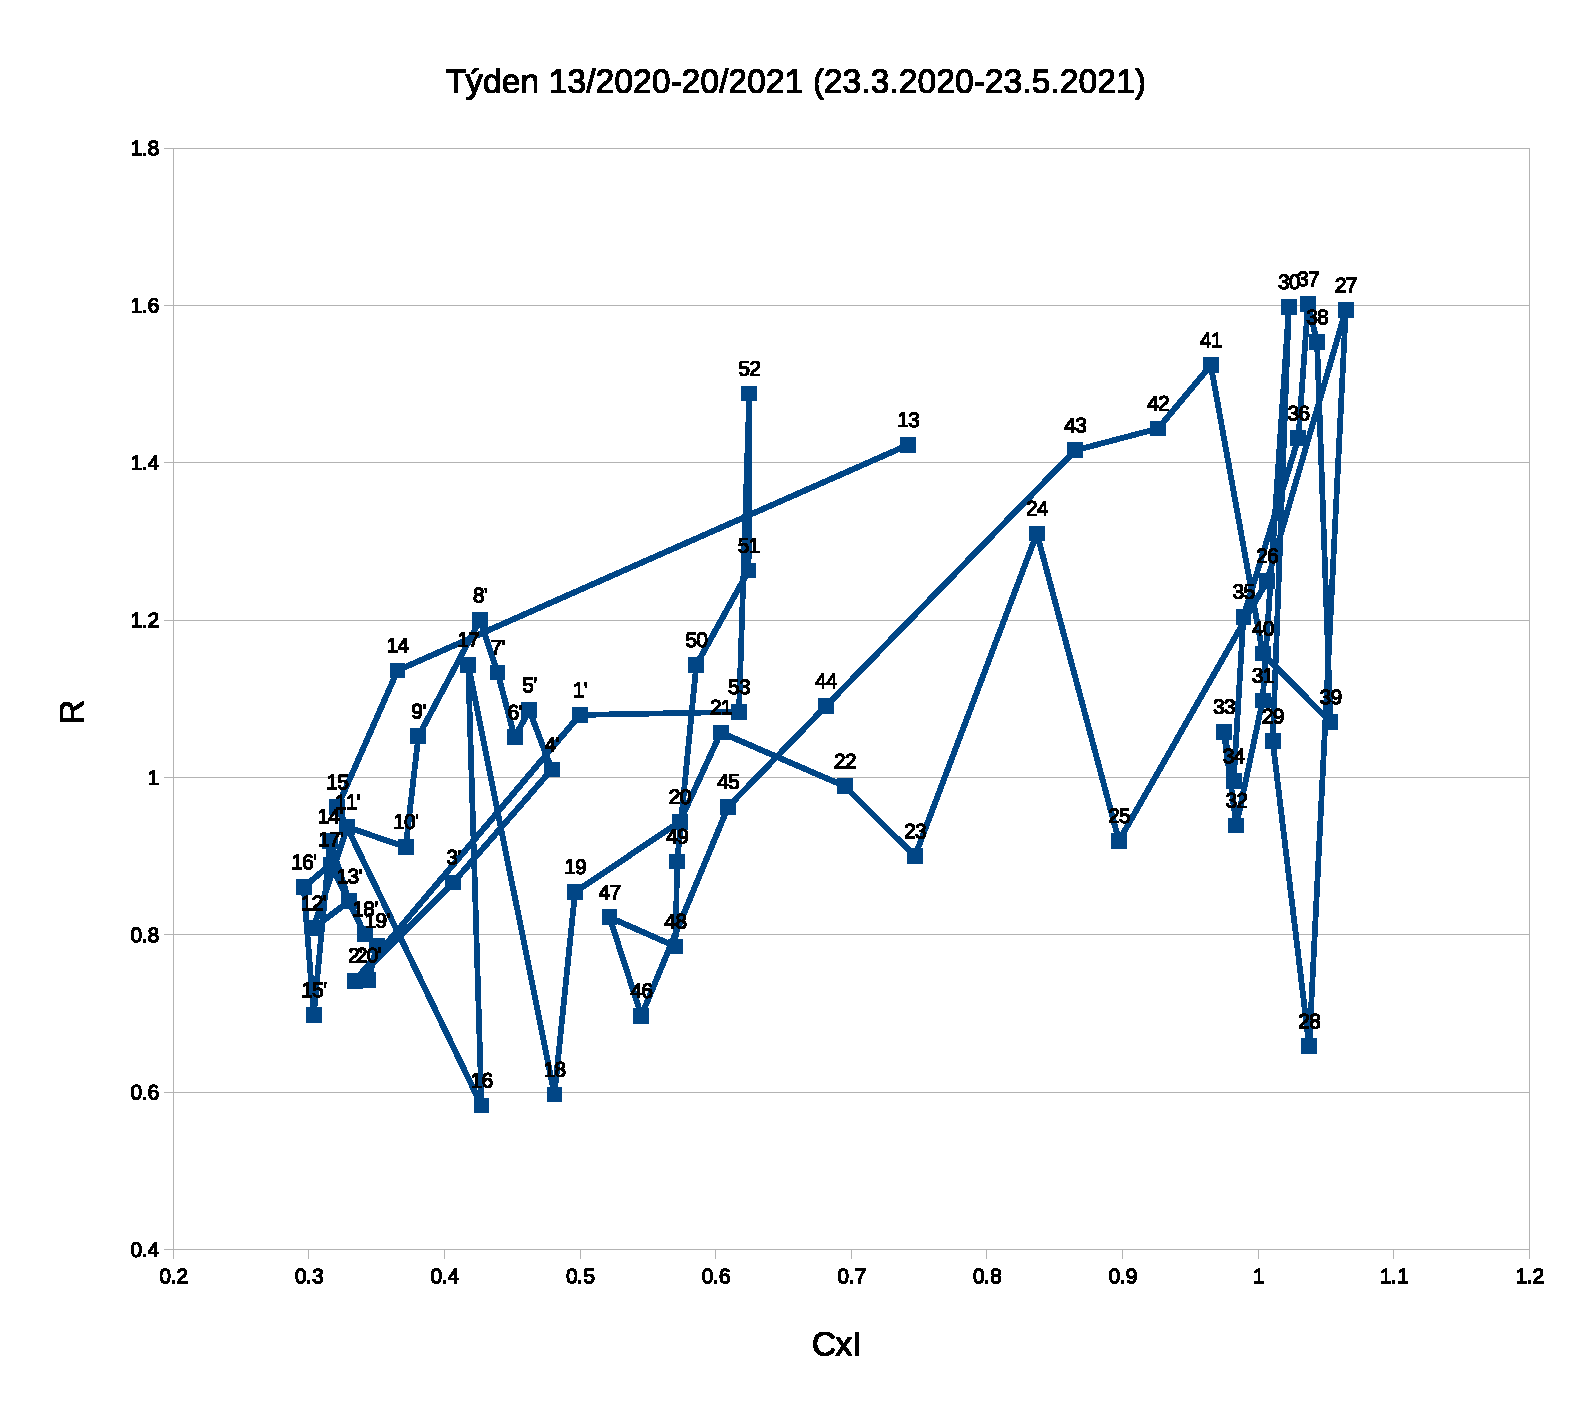
\includegraphics[scale=0.4]{pic/epi}
\caption{Závislost $R_t$ na $C_{t-2} \times I_t$. Hodnoty u~jednotlivých bodů označují čísla týdnů, ze kterých pochází $R$, apostrof označuje rok 2021.}
\label{fig:xy}
\end{center}
\end{figure}
Jakkoli v~grafu není příliš patrná žádná funkční závislost, vykreslení analogických grafů 
pro vhodně zvolené časové úseky vykazuje 
zřetelnější strukturu, jak je ukázáno na obrázku \ref{fig:xy5}
\begin{figure}
\begin{center}
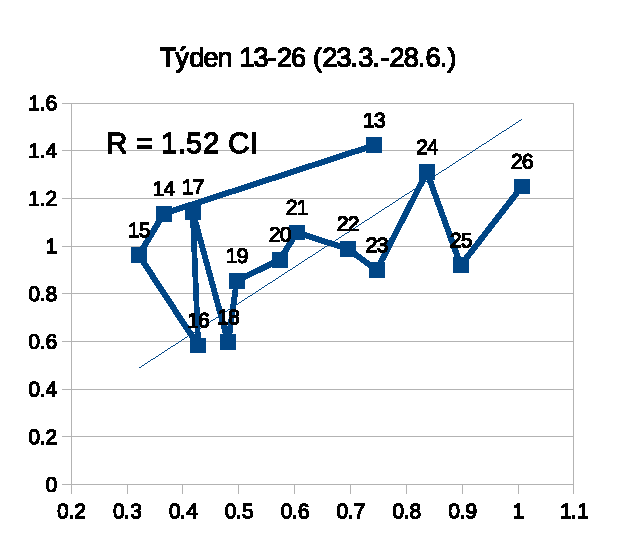
\includegraphics[scale=0.35]{pic/g1}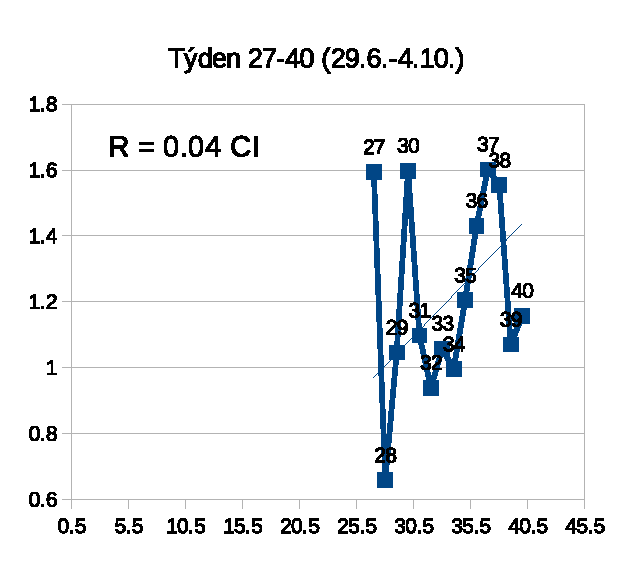
\includegraphics[scale=0.35]{pic/g2}
\\
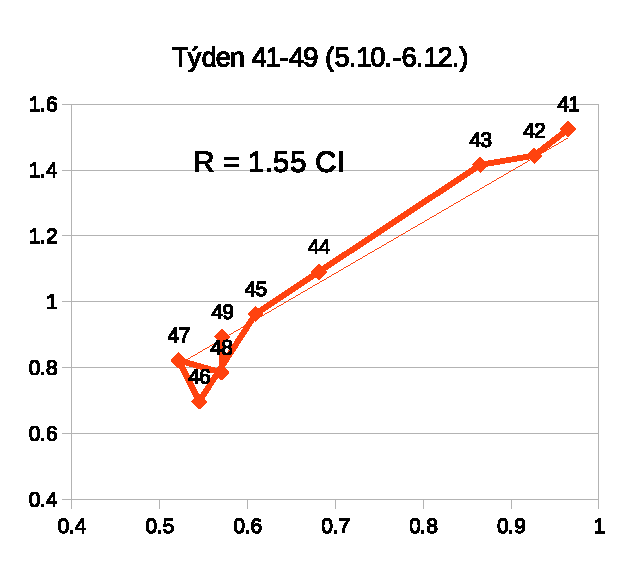
\includegraphics[scale=0.35]{pic/g3}
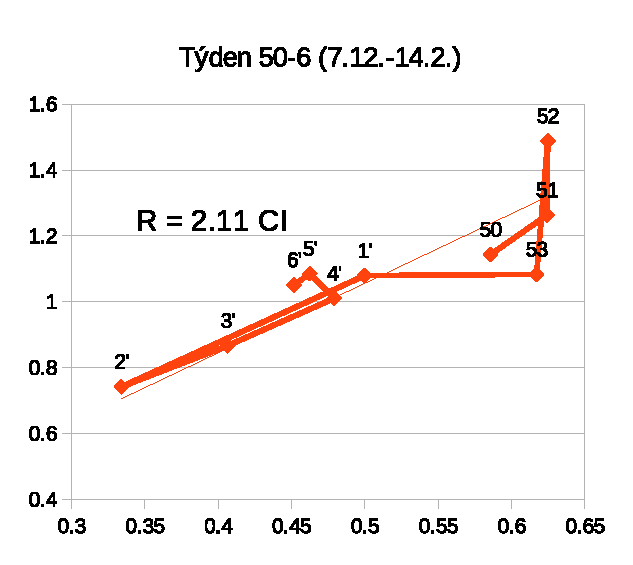
\includegraphics[scale=0.35]{pic/g4}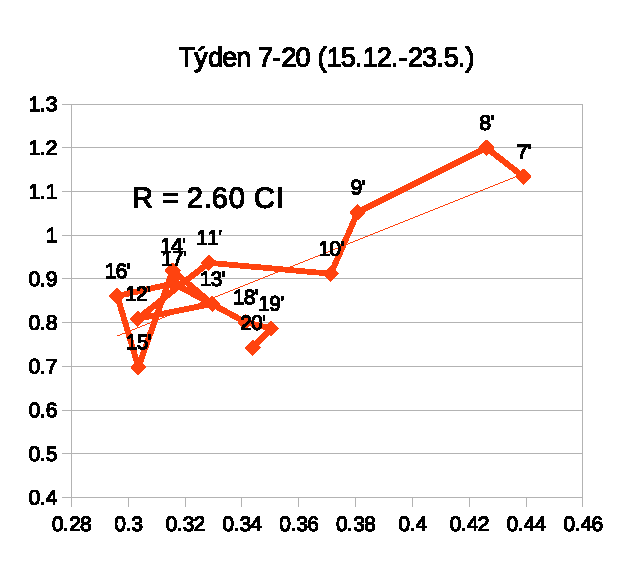
\includegraphics[scale=0.35]{pic/g5}
\caption{Závislost $R_t$ na $C_{t-2} \times I_t$ v~různých časových úsecích epidemie.}
\label{fig:xy5}
\end{center}
\end{figure}
Na všech grafech kromě druhého, odpovídajícího letním měsícům, je patrná lineární závislost (trend
vždy prochází počátkem), což svědčí pro platnost
modelu (\ref{eq:r}) s~po částech konstantním $r$. Proti tomu lze sice namítnout,
že rozdělení na úseky bylo učiněno až na základě znalosti dat, takže zjištěná závislost může být i dílem náhody, na druhou stranu je závislost v~rámci úseků poměrně přesná, přičemž některé větší výkyvy lze vysvětlit: například ty v~52. a 53.
týdnu jsou vysvětlitelné zavedením antigenních testů pro veřejnost,
která skokově zvýšila počty odhalených infekcí. 

Ačkoli výše diskutovaný postup není ve striktním souladu se zásadou matematického modelování, že struktura modelu musí být navržena ještě bez znalosti dat, dále předpokládáme v~každém úseku konstantní hodnotu $r_{t}$,
danou příslušným lineárním trendem, čímž dojdeme k~modelu $r_{t}$ znázorněnému na obrázku \ref{fig:model}.
\begin{figure}
\begin{center}
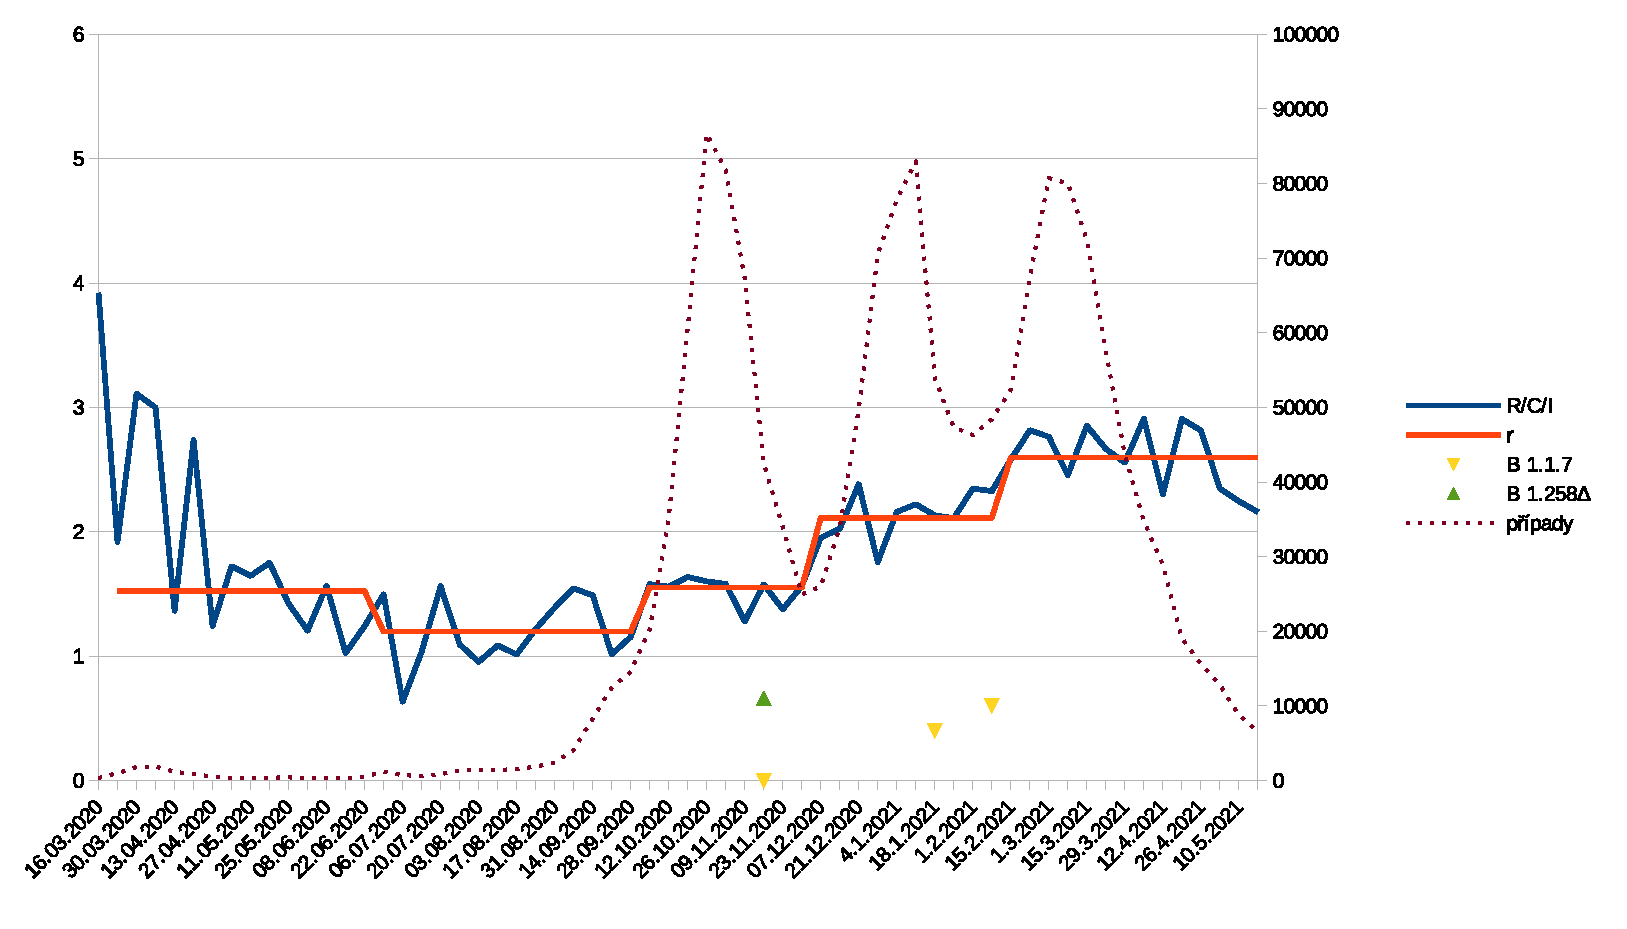
\includegraphics[scale=0.4]{pic/whole}
\caption{Navržený model $r_t$ (červená), odhad $r_t$ pomocí $\hat{r}_t = \frac{R_{t}}{C_{t-2}I_{t}}$ (modrá), procentní poměr varianty B.1.1.7 alfa (žluté trojúhelníky), procentní poměr „české varianty“ B1.258$\Delta$ (zelený trojúhelník), počty hlášených případů za týden (tečkovaná čára, pravá osa).}
\label{fig:model}
\end{center}
\end{figure}
Kromě našeho modelu $r_t$ graf zobrazuje jeho odhad $\hat r_t$, dále průběh epidemie a poněkud kusé a pravděpodobně málo spolehlivé informace o~procentním zastoupení takzvané
české varianty B.1.258$\Delta$ a varianty B.1.1.7, nově označované jako varianta alfa:
\begin{itemize}
\item odhady \cite{brejova2021b}, že v~listopadu byla
prevalence varianty alfa nulová a prevalence „české“ varianty 60\%, 
\item zmínku tehdejšího ministra zdravotnictví Blatného z~22. ledna, že britská mutace tvoří 40\,\% vzorků (\cite{blatnybrigit}).
\item výzkumnou zprávu \cite{diana}, která 19. února odhaduje rozšíření varianty alfa
na přibližně 60\,\%.
\end{itemize}
To vše naznačuje, že každá vlna epidemie odpovídá jedné úrovni základního reprodukčního čísla, případně jedné převládající variantě viru. Potvrzení této hypotézy by však vyžadovalo
mnohem přesvědčivější evidenci.

Jakkoli vypadá náš model $r_t$ realisticky, neodpovídá na otázku, která z~jeho složek se v~čase mění: zda základní reprodukční číslo $R^0$ nebo míra dodatečné ochrany $P$. Když však odhlédneme od léta 2020, je křivka $r_t$ rostoucí a její nárůst mezi prvním půlrokem epidemie a jarem 2021 zhruba odpovídá udávanému nárůstu nakažlivosti varianty alfa proti původní variantě (viz níže), zdá se tedy pravděpodobnější, že příčinou nárůstu je změna základního reprodukčního čísla, způsobená nástupem nových mutací. Předpoklad, že $P$ je konstantní, je přitom do jisté míry 
oprávněný, neboť za celé sledované období s~výjimkou léta
2020 platila povinnost nosit roušky, a například z~výzkumu \cite{paqcovid}
vyplývá, že poměr rizikových kontaktů s~rouškou a bez roušky se
v~čase příliš nemění. 

\section*{Výsledky}

V~této sekci se pokusíme odhadnout míru vakcinace nutnou pro udržení
klesajícího trendu epidemie pro několik scénářů budoucího vývoje. 

K~23. květnu 2021 bylo první dávkou vakcíny naočkováno 3273 tisíc
občanů, z~toho 1067 tisíc i druhou dávkou. což odpovídá zhruba 31\,\%,
respektive 10\,\% populace (36\,\%, respektive 12\,\% z~těch, u~kterých nebyla
dosud hlášena infekce). Tyto hodnoty spolu s~naším odhadem účinnosti
odpovídají míře ochrany vakcínou $v=0.27$. Dále bylo k~tomuto dni
hlášeno 1658 tisíc případů infekce, což při $\alpha=0.4$ znamená
4145 tisíc přirozeně imunních, tedy 38\,\% populace. To dle (\ref{eq:i})
dohromady dává $I=0.45$. Náš odhad současné hodnoty $r$ je $2.6$ (viz obrázek \ref{fig:model}), což znamená, že pro udržení $R=1$ je potřeba redukce kontaktů
$C=\frac{1}{r\times I}=0.85$. Pokud bychom požadovali, aby $R=0.8$,
pak by muselo být $C=0.68$. Hodnota $C$ odpovídající danému týdnu
podle \cite{paqcovid} je přitom 0.69, což by mělo spolu
s~rychle rostoucí proočkovaností a předpokládaným snižováním rizikových kontaktů v letních měsících, daným absencí kontaktů ve školách, stačit k~udržení znatelného poklesu.

Stavu, kdy by nebylo nutno kontakty redukovat a přitom by bylo $R=1$,
pak odpovídá $v=1-\frac{R}{(1-x/\alpha)r_{t}}=0.41$, čehož by bylo dosaženo, kdyby bylo 38\,\% celé populace očkováno oběma dávkami nebo
například $45\,\%$ první a $12\,\%$ druhou dávkou.

Je nutno si uvědomit, že tato čísla platí \emph{ceteris peribus},
to jest za podmínky, že všechny ostatní proměnné zůstanou stejné, což do budoucnosti není nijak zaručeno.
Toto se týká zejména míry ochranných opatření $P_{t}$, o~které jsme zatím
předpokládali, že se v~čase nemění. Pokud by se však například
naráz přestaly nosit roušky a respirátory, jistě by to znamenalo nárůst
reprodukčního čísla. Kdybychom před\-po\-klá\-da\-li 50\%
účinnost této ochrany a spolu s~\cite{paqcovid} její 50\% současné
použití, pak by její plošné vynechání zvětšilo $r$ o~33\,\%,\footnote{Při 50\% kontaktech a 50\% účinnosti s~rouškou je $r=(0.5+0.5\times0.5)r^{\star}$,
kde $r^{\star}$ je analogie veličiny $r$ neuvažující ochranu úst.} což by samozřejmě zvýšilo nutnou míru vakcinace. Totéž platí v~případě,
že by místo současné pře\-vlá\-da\-jí\-cí mutace převládla 
varianta B.1.617 nově nazývaná delta (dříve indická varianta), o~které se všeobecně předpokládá, že je nakažlivější,
viz \cite{ecdc2021india}. 

V~tabulce \ref{tab:res} je uvedena nutná restrikce kontaktů (při současné
míře pro\-oč\-ko\-va\-nos\-ti) a nutná míra vakcinace pro dvě cílové hodnoty
$R=1$ a $R=0.8$, a to pro 
současnou hodnotu $r$ a její o~50\,\% vyšší hodnotu, o~které předpokládáme, že odpovídá variantě delta. Pro oba případy jsou uvedeny hodnoty bez vysazení a~s~vy\-sa\-zením roušek. Pro každý scénář a každé
cílové $R$ uvádíme dvě možnosti, jak pomocí očkování zajistit potřebnou ochranu:
proočkovanost všech oběma dávkami (sloupec $\pi$) a rozdílnou proočkovanost
první a druhou dávkou ($\pi^{1}$ a $\pi^{2})$ s~tím, že očkovanost první dávkou naroste ze současného stavu o~stejnou hodnotu jako naočkovanost druhou dávkou.
\begin{table}
\begin{center}
\begin{tabular}{l|c|c|ccc|ccc}									 Cílové $R$	& $1$	& $0.8$	& $1$	&	&	& $0.8$	&	&	\\  Dosaženo změnou	& $C$	& $C$	& $\pi$	& $\pi_1$	& $\pi_2$	& $\pi$	& $\pi_1$	& $\pi_2$	\\ \hline Květen '21 ($r=2.6$)	& $0.85$	& $0.68$	& $0.38$	& $0.45$	& $0.12$	& $0.5$	& $0.7$	& $0.25$	\\ ... bez roušek ($r=3.47$)	& $0.64$	& $0.51$	& $0.53$	& $0.59$	& $0.38$	& $0.62$	& $0.68$	& $0.47$	\\ Nová varianta ($r=3.9$)	& $0.57$	& $0.46$	& $0.58$	& $0.64$	& $0.43$	& $0.67$	& $0.72$	& $0.51$	\\ ... bez roušek ($r=5.2$)	& $0.43$	& $0.34$	& $0.69$	& $0.74$	& $0.53$	& $0.75$	& $0.8$	& $0.6$	\\ 
\end{tabular}		
\caption{Nutná míra redukce kontaktů a proočkovanosti pro dosažení cílového $R$. $C$ -- nutná míra redukce kontaktů při proočkovanosti k~23. 5. 2020, $\pi$ -- proočkovanost celé populace oběma dávkami za předpokladu, že všichni mají obě dávky. $\pi_1$ a $\pi_2$ -- jedna z~možností kombinace proočkovanosti celé populace první, respektive druhou dávkou (nepředpokládá se redukce kontaktů). }							 	 
\label{tab:res}
\end{center}

\end{table}


\section*{Diskuse}

V~předchozím odstavci jsme uvedli řadu kvantitativních výsledků, je
však nutno připomenout, že jsou tato čísla založena na jednoduchém
modelu a -- což je ještě důležitější -- na některých parametrech,
jejichž odhad je nepřesný. Nejzávažnějším je tento problém pro parametr
$\alpha$ -- procento odhalených případů -- jehož hodnotu je velice
těžké odhadnout.\footnote{Základní problém jejího odhadu je ten, že se epidemie zhruba řídí
lineárními diferenciálními (či diferenčními) rovnicemi, jimž (případně
s~jinými koeficienty) vyhovují libovolné násobky jejich řešení. Pokud
například pozorujeme polovinu případů, našemu modelu bude vyhovovat
i hypotéza, že pozorujeme všechny.} K~našemu odhadu $\alpha=0.4$ jsme došli třemi způsoby: na základě výzkumu
\cite{paqcovid}, na základě procenta záchytů v~nemocnicích a na základě poměru infekčnosti
variant. 

Konkrétně, podle \cite{paqcovid} poměr osob, u~nichž existovalo riziko
nákazy nebo pociťovaly příznaky typické pro covid-19 a přitom byly testovány,
činil cca 20\,\% v~září, cca 40\,\% začátkem března a až koncem března
vyšplhal tento poměr na cca 60\,\%, což v~průměru odpovídá naší volbě $\alpha.$
Jako další nápověda pro náš odhad sloužil podíl hospitalizovaných,
kteří byli před hospitalizací detekováni, jeho komplement donedávna sloužil jako
jeden z~komponentů indexu rizika protiepidemického systému PES \cite{PES}. Tato hodnota přitom může sloužit jako horní odhad $\alpha$.\footnote{Dle Bayesova vzorce 
\[
\alpha=\mathrm{P}[\text{detekován}|\text{hospitalizován}]\frac{\mathrm{P}[\text{hospitalizován}]}{\mathrm{P}[\text{hospitalizován}|\text{detekován}]}
\]
\cite{Pribylova2021Model}). Pokud přirozeně předpokládáme, že hospitalizace
je pozitivně korelována s~detekcí, bude zlomek menší než jedna,
což znamená že $\alpha$\textless P{[}detekován\textbar hospitalizován{]}. } 
Podíl detekovaných hospitalizovaných v~lednu činil okolo 0.45 a až od března se ustálil
na hodnotách okolo 60\,\%, což víceméně odpovídá výsledkům \cite{paqcovid}. 
Pro námi zvolenou hodnotu $\alpha=0.4$ navíc svědčí náš model, který na základě této hodnoty dochází k~podílu $1.68$ současného a zářijového základního reprodukčního čísla, což například není daleko od hodnoty $1.78$ uvedené v~\cite{curran2021transmission}. 

Vědomi si nejistoty odhadu $\alpha$ a faktu, že se v~mediálním prostoru spekulovalo o~mnohem vyšších podílech neodhalených infekcí, než by odpovídalo $\alpha=0,4$ provedli
jsme v~rámci citlivostní analýzy stejné výpočty jako v~předchozím
odstavci, ovšem pro $\alpha=0,25$. Při této hodnotě by získanou
imunitu v~současné době mělo přibližně 6,5 milionu osob na rozdíl od 4,05
v~případě $\alpha=0,4$. Potřebné míry redukce kontaktů a očkovanosti uvádíme na obrázku \ref{fig:calpha}.

\begin{figure}
\begin{center}
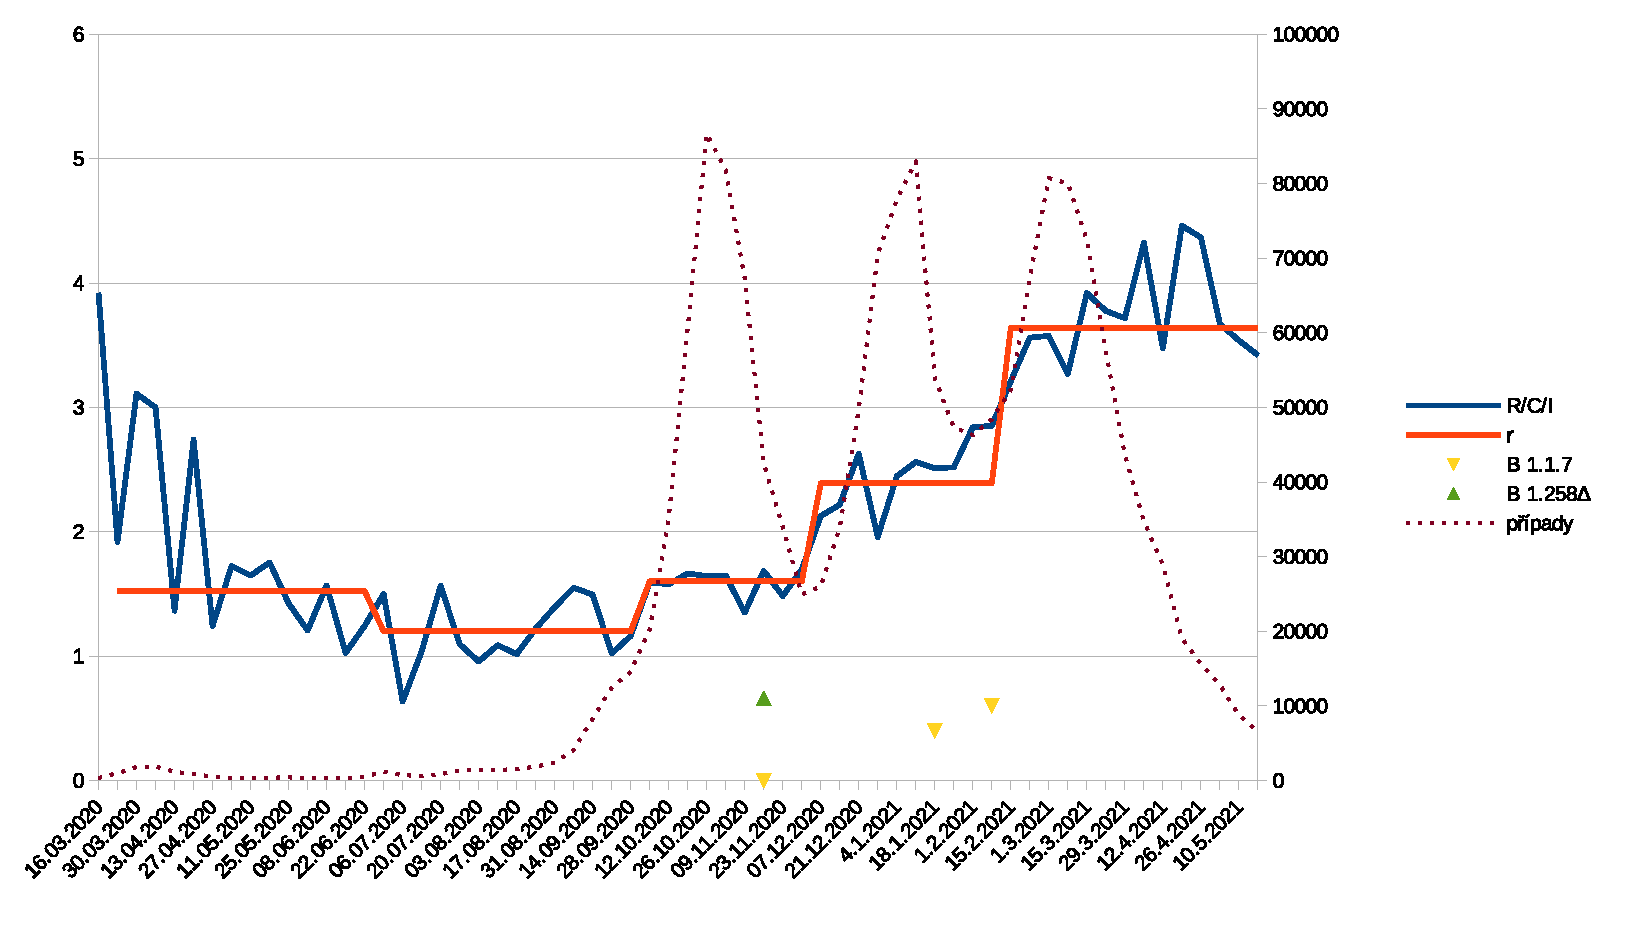
\includegraphics[width=10cm]{pic/whole4}
						 

\begin{tabular}{l|c|c|ccc|ccc}									
Cílové $R$	& $1$	& $0.8$	&	&	&	& $0.8$	&	&	\\ 
Dosaženo změnou	& $C$	& $C$	& $\pi$	& $\pi_1$	& $\pi_2$	& $\pi$	& $\pi_1$	& $\pi_2$	\\ \hline
Květen '21 ($r=3.67$)	& $0.96$	& $0.77$	& $0.3$	& $0.3$	& $0.05$	& $0.44$	& $0.58$	& $0.19$	\\
...bez roušek ($r=4.89$)	& $0.72$	& $0.58$	& $0.47$	& $0.53$	& $0.32$	& $0.58$	& $0.63$	& $0.43$	\\
Nová varianta ($r=5.51$)	& $0.64$	& $0.51$	& $0.53$	& $0.58$	& $0.38$	& $0.62$	& $0.68$	& $0.47$	\\
... bez roušek ($r=7.34$)	& $0.48$	& $0.38$	& $0.65$	& $0.7$	& $0.49$	& $0.72$	& $0.77$	& $0.56$	
\end{tabular}									


\caption{Citlivostní analýza: $\alpha=0.25$. Vysvětlivky viz obrázek \ref{fig:model} a tabulku \ref{tab:res}}
\label{fig:calpha}
\end{center}
\end{figure}
Z~výsledků je vidět, že ani o~2.45 milionu větší promořenost situaci příliš
nepomohla. Požadavky na současnou redukci kontaktů jsou sice znatelně
nižší, požadavky na vakcinaci jsou však srovnatelné. Vysvětlení, proč
tomu tak je, je nasnadě: pokud je více imunních lidí, pak proto,
aby se dosáhlo stejných počtů nakažených, musí být značně vyšší $r_{t}$
-- zde je to 3.67 místo 2.6 -- což pochopitelně vyžaduje pro stejné $R$
větší proočkovanost. Poměr reprodukčního čísla varianty alfa a
původní varianty však v~tomto případě vychází 2.27, což je oproti
existujícím odhadům značně nadsazené -- zdá se tedy, že vyšší hodnota
$\alpha=0.4$ je realističtější.

Další slabina našeho modelu může spočívat v~nejistotě týkající se účinnosti vakcíny
-- odhady z~\cite{Hall_etal2021} mají poměrně velké konfidenční
intervaly, a například novější, byť nerecenzovaná studie \cite{Shapiro_etal2021}
uvádí značně větší účinnosti: $e^{1}=0.82$, $e^{2}=0.942$. Výsledky pro tyto hodnoty jsou vidět na obrázku \ref{fig:cv}. Podobně jako v~předchozím případě vidíme, že požadavky na vakcinaci jsou mírnější, ne však řádově.

\begin{figure}
\begin{center}
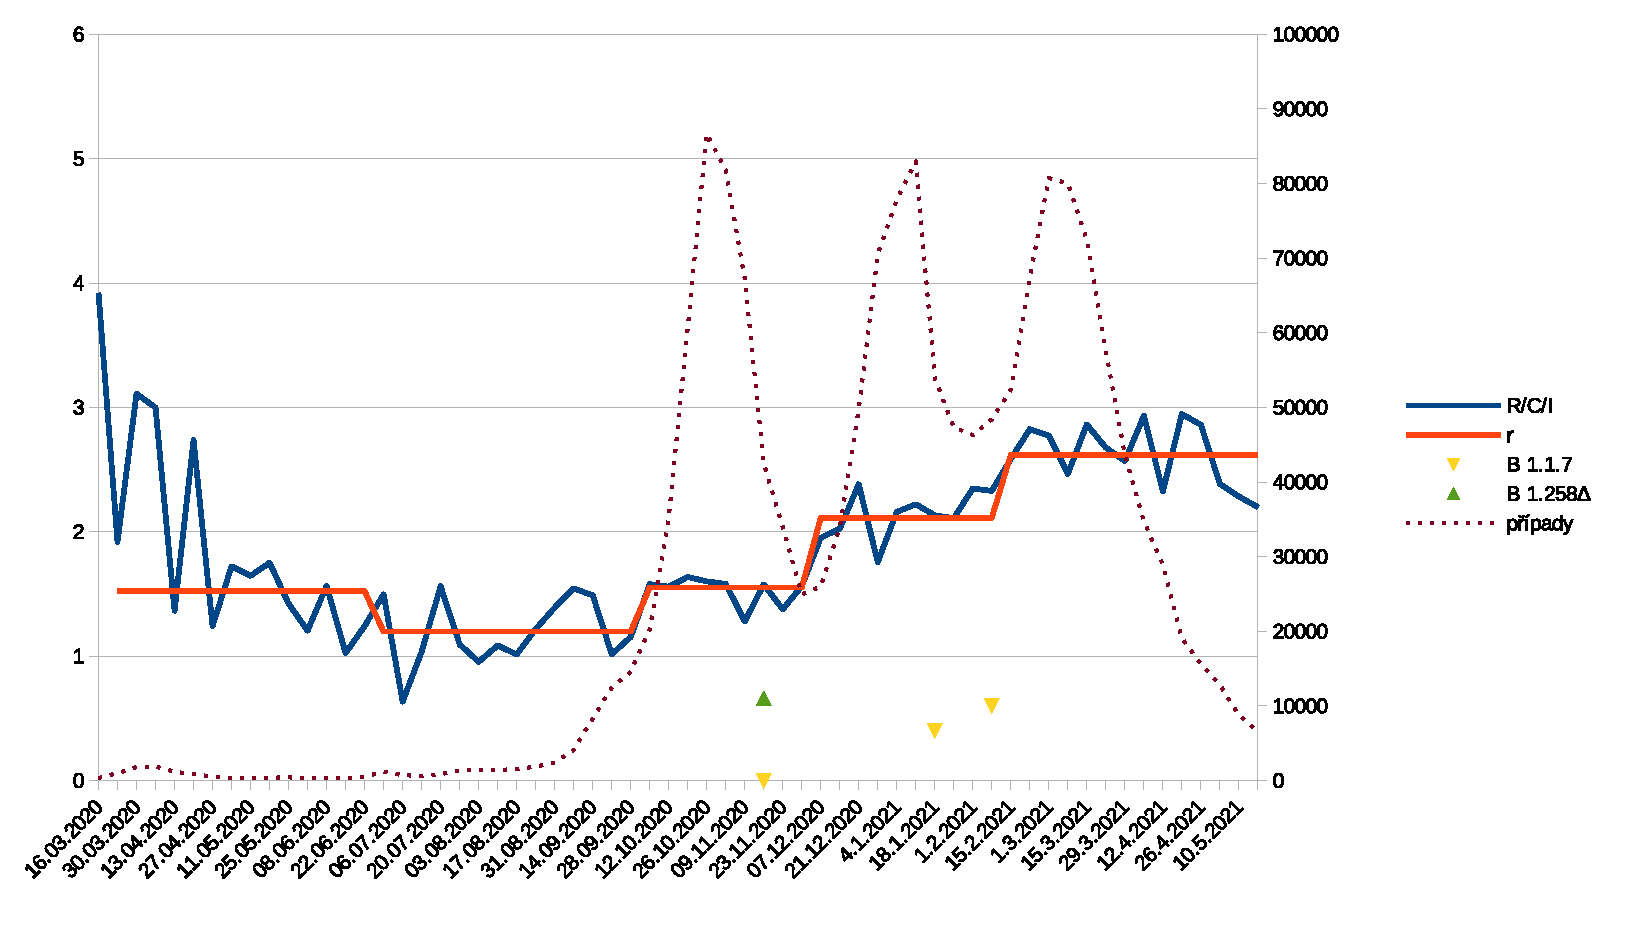
\includegraphics[width=10cm]{pic/wholee} 

\begin{tabular}{l|c|c|ccc|ccc}									
Cílové $R$	& $1$	& $0.8$	&	&	&	& $0.8$	&	&	\\ 
Dosaženo změnou	& $C$	& $C$	& $\pi$	& $\pi_1$	& $\pi_2$	& $\pi$	& $\pi_1$	& $\pi_2$	\\ \hline
Květen '21 ($r=2.65$)	& $0.89$	& $0.71$	& $0.35$	& $0.37$	& $0.08$	& $0.46$	& $0.59$	& $0.19$	\\
... bez roušek ($r=3.53$)	& $0.66$	& $0.53$	& $0.49$	& $0.53$	& $0.32$	& $0.57$	& $0.61$	& $0.4$	\\
Nová varianta ($r=3.98$)	& $0.59$	& $0.47$	& $0.53$	& $0.57$	& $0.37$	& $0.61$	& $0.65$	& $0.44$	\\
... bez roušek ($r=5.3$)	& $0.44$	& $0.35$	& $0.62$	& $0.66$	& $0.46$	& $0.68$	& $0.72$	& $0.51$
\end{tabular}									

\caption{Citlivostní analýza: $e^{1}=0.82$, $e^{2}=0.942.$ Vysvětlivky viz obrázek \ref{fig:model} a tabulku \ref{tab:res}}
\label{fig:cv}

\end{center}
\end{figure}


Další námitkou vůči našemu modelu, již dříve diskutovanou, může být to, že nebere v~úvahu sezonní
vlivy. Byť dle našich znalostí zatím v~tomto směru neexistuje přesvědčivá vědecká
evidence, obecně se soudí, že se virus v~létě šíří pomaleji, ať už
je to kvůli slunečnímu záření nebo proto, že se lidé setkávají více
pod širým nebem. Pokles v~létě 2020, který jsme přisoudili absenci
komunitního šíření, by alespoň částečně mohl být důsledkem právě tohoto
efektu. Proto jsme jako další případ citlivostní analýzy svůj model modifikovali tak, aby kromě dosavadních determinant reprodukční číslo záviselo
také na periodické složce: konkrétně jsme modifikovali (\ref{eq:r}) na 
$r_{t}=R_{0}^{t}\times P_{t}\times(1+\kappa\phi_{t})$, kde $\phi_{t}$
je sinusoida s~roční periodou a maximem v~půli ledna a $\kappa$ je
parametr, který jsme určili minimalizací střední čtvercové chyby
(s~vypuštěním letních pozorování). Výsledky jsou zobrazeny na obrázku \ref{fig:cc}

\begin{figure}

\begin{center}

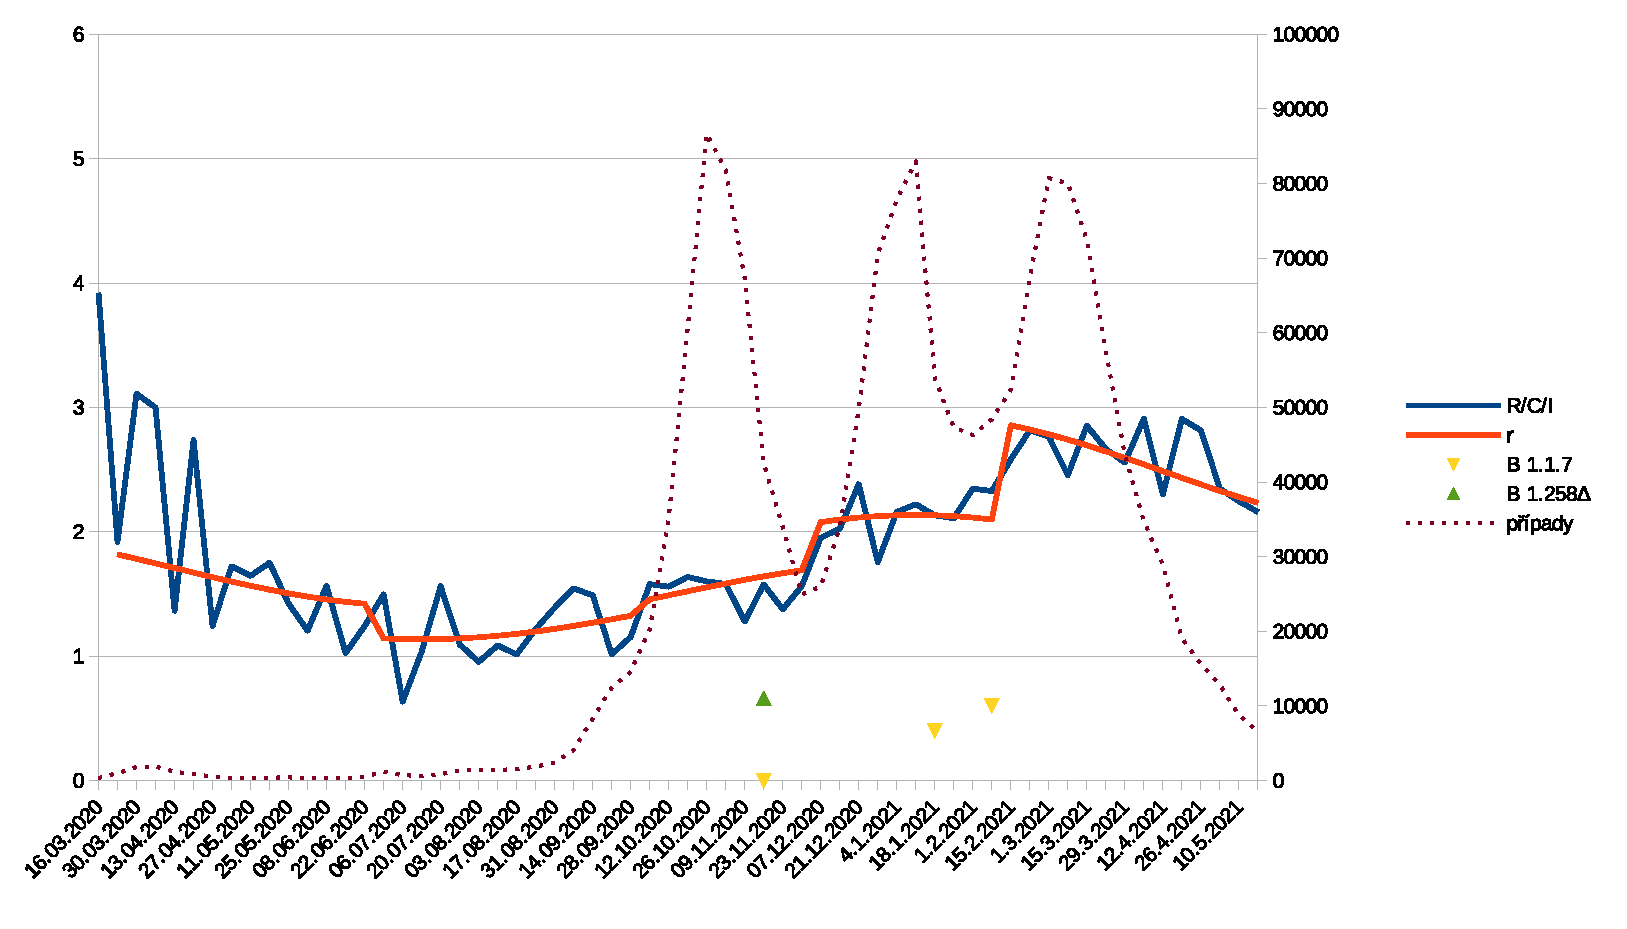
\includegraphics[width=10cm]{pic/wholec} 

\begin{tabular}{l|c|c|ccc|ccc}									
Cílové $R$	& $1$	& $0.8$	&	&	&	& $0.8$	&	&	\\ 
Dosaženo změnou	& $C$	& $C$	& $\pi$	& $\pi_1$	& $\pi_2$	& $\pi$	& $\pi_1$	& $\pi_2$	\\ \hline
Květen '21 ($r=2.25$)	& $0.99$	& $0.79$	& $0.28$	& $0.26$	& $0.03$	& $0.42$	& $0.55$	& $0.17$	\\
... bez roušek ($r=3$)	& $0.74$	& $0.59$	& $0.46$	& $0.51$	& $0.31$	& $0.57$	& $0.62$	& $0.41$	\\
Nová varianta ($r=3.38$)	& $0.66$	& $0.53$	& $0.52$	& $0.57$	& $0.37$	& $0.61$	& $0.67$	& $0.46$	\\
... bez roušek ($r=4.5$)	& $0.49$	& $0.39$	& $0.64$	& $0.69$	& $0.49$	& $0.71$	& $0.76$	& $0.56$	\\
... v~lednu ($r=6.03$)	&	&	& $0.73$	& $0.78$	& $0.58$	& $0.78$	& $0.84$	& $0.63$	\\
\end{tabular}									


\caption{Citlivostní analýza: cyklická složka. Vysvětlivky viz obrázek \ref{fig:model} a tabulku \ref{tab:res}}
\label{fig:cc}
\end{center}

\end{figure}
Jak se dalo očekávat, požadavky jsou zde měkčí než v~základní variantě,
byť opět nikoli řádově. Nicméně je zde potřeba vzít v~úvahu i fakt, že  pokud model se sezónní složkou platí, nacházíme se v~současné době blízko dna cyklické složky, přičemž na jejím předpokládaném
vrcholu v~lednu 2022 by veličina $r$ byla o~33\,\% vyšší, což by například
v~nejhorším scénáři z~tabulky znamenalo požadavek 73\% místo 64\% proočkovanosti
pro udržení $R=1$, viz poslední řádek tabulky.

\section*{Závěr}

Naše výsledky přesvědčivě ukazují, že by v~současné době neměl být problém epidemii
utlumit a už při cca 60\% proočkovanosti
by bylo možno zrušit většinu restriktivních opatření včetně nošení roušek. Přitom dle \cite{paqcovid} v~současné době 64\,\% dospělých respondentů uvádí, že jsou očkováni nebo ochotni nechat se očkovat, což znamená 56\,\% celé populace, pokud by se jako v~současnosti očkovali pouze lidé starší 16 let, případně 59\,\% populace, pokud by se stejnou měrou očkovaly i děti od 12 let. Dosažení těchto hranic není úplně nerealistické, a to ani
ani z~hlediska logistiky (viz kapitolu \ref{Logistika_ockovani}). Hlavní nebezpečí se tedy
skrývá v~možném nástupu nové varianty, přičemž je potřeba si uvědomit,
že importovaná varianta je schopna v~situaci, kdy je ostatních
případů málo, velice rychle převládnout. Scénář importu některé
nové varianty v~průběhu prázdnin, až se lidé budou vracet z~dovolených, je
tedy bohužel poměrně reálný.

Dá se předpokládat, že klíčový pro další vývoj epidemie bude začátek podzimu. Tou dobou budou pro potřebnou míru proočkovanosti naše výsledky stále do jisté míry platit: přirozeně imunizovaných sice bude o~něco více, ale ne o~mnoho, protože přes léto budou čísla nakažených pravděpodobně velice nízká. Platit budou i při uvažování sezónního vlivu, protože sezónní křivka bude přibližně ve stejném bodě jako dnes. 

Při velmi pravděpodobném scénáři importu nové varianty budou platit čísla z~druhého a třetího řádku výsledných tabulek, což pro život bez roušek ve všech případech vyžaduje $60-70\%$ proočkovanost celé populace, tedy $70-80\,\%$ obyvatel nad 16 let, pokud se nebudou očkovat děti nad 12 let, případně $65-75\,\%$ obyvatel nad 12 let, pokud by se tyto děti očkovaly. Vzhledem k~současné situaci se dosažení takto vysoké proočkovanosti bohužel nezdá příliš realistické. Naše odhady jsou přitom optimistické v~tom smyslu, že neuvažují vyvanutí imunity, ať už té získané proděláním nemoci či očkováním.
Pokud tedy nebudeme chtít nuceně opět sáhnout k~plošným
opatřením, jedinou možností obrany před tímto scénářem je posílení
dodatečné ochrany $P$, zejména pak testování a trasování, které tím, že
infekčního jedince včas izolují, mohou mít na reprodukční číslo značný
vliv.